%-----------------------------------------------------------------------------%
\chapter{\babDua}
\label{bab:2}
%-----------------------------------------------------------------------------%
Untuk memulai penelitian, dibutuhkan kerangka berpikir yang sesuai untuk permasalahan yang ingin dipecahkan. Untuk membentuk kerangka berpikir yang sesuai, perlu dikaitkan dengan hasil studi literatur yang telah dilakukan. Oleh karena itu, pada bab ini, dijelaskan hasil studi literatur yang telah dilakukan yang telah dikaitan dengan kerangka kerja untuk penelitian ini.


\section{\textit{Blockchain}}
\label{sec:litblockchain}

\textit{Blockchain} adalah teknologi \textit{ledger} terdistribusi dan terdesentralisasi. Karakteristik utama dalam \textit{blockchain} adalah \textit{tamper evident} yaitu terdapat catatan atas semua perubahan data yang terjadi pada \textit{datledger}; dan \textit{tamper resistant} yaitu kebal terhadap perubahan data secara tidak sah. \textit{Data temperance} dicegah dengan mencatat semua transaksi dalam bentuk \textit{block} dan setiap \textit{block} memiliki \textit{timestamp} dan memiliki nilai \textit{hash} pada \textit{block} sebelumnya, membentuk rantai (\textit{chain}). \citep{Ahmed2020} \citep{Yaga2018}. 

Terdapat dua tipe \textit{blockchain}. Yang pertama adalah \textit{public permissionless blockchain}, di mana siapapun dapat berpartisipasi dalam jaringan, melihat semua transaksi, bergabung dalam konsensus, serta melakukan transaksi. Contoh \textit{blockchain} dengan tipe ini adalah Bitcoin dan Ethereum. Dikarenakan siapapun dapat menerbitkan \textit{block}, perlu dilakukan konsensus untuk menjaga integritas sistem serta mencegah pengguna jahat untuk merusak ataupun memalsukan transaksi \citep{Yaga2018}.

Tipe kedua yaitu \textit{private permissioned blockchain}, di mana hanya pihak yang terdaftar dapat berpartisipasi dalam jaringan. Dalam \textit{permissioned blockchain} terdapat otoritas yang mengatur keanggotaan, siapa saja yang dapat menerbitkan \textit{block}, serta dapat membatasi akses ke \textit{resource} tertentu. Berbeda dengan \textit{permissionless blockchain}, semua anggota \textit{permissioned blockchain} memiliki identitas dan dikenali oleh anggota lainnya. Hal ini membuat model ini menggunakan asumsi \textit{trust} pada anggota lainnya, tidak seperti pada \textit{permissionless blockchain}. Mekanisme konsensus pada tipe ini umumnya lebih efisien dibandingkan dengan konsensus pada \textit{permissionless blockchain} dikarenakan setiap anggota memiliki identitas yang jelas. Transaksi pada tipe \textit{blockchain} ini tetap diproses secara desentralisasi serta setiap anggota tetap memiliki salinan \textit{ledger} di penyimpanan lokal masing-masing \citep{Yaga2018}.


\subsection{Konsensus pada \textit{Blockchain}}
\label{subsec:consensus}

\textit{Blockchain} berjalan tanpa otoritas sentral (kecuali pada \textit{permissioned blockchain}) sehingga mengandalkan mekanisme konsensus untuk menjaga operasional dan integritas sistem. Konsensus merupakan metode validasi transaksi yang ditentukan dan disetujui oleh seluruh anggota \textit{blockchain} untuk mendapatkan \textit{trust}. Terdapat berbagai mekanisme konsensus antara lain Proof-of-Work, Proof-of-Stake, Delegated Proof of Stake, Byzantine Fault Tolerance, dan masih banyak lagi \citep{Ahmed2020}. 

Proof-of-Work adalah mekanisme konsensus paling umum digunakan pada \textit{blockchain}. Proof-of-Work melibatkan anggota \textit{blockchain} untuk memecahkan teka-teki \textit{cryptographic} untuk membuat sebuah \textit{block}. Kegiatan ini dinamakan \textit{mining} dan pelakunya dinamakan \textit{miner}. Dalam Proof-of-Work, setiap anggota mencari sebuah \textit{nonce} yang dijadikan sebagai input fungsi \textit{hash} selain daftar transaksi-transaksi pada sistem \textit{blockchain}. Suatu \textit{block} dikatakan valid apabila nilai \textit{hash} pada \textit{block} tersebut memenuhi syarat yaitu memiliki \textit{leading zeroes} yang telah disepakati. \textit{Block} tersebut kemudian dikirim ke anggota jaringan lainnya untuk dilakukan validasi. \textit{Miner} yang dapat menemukan \textit{block} paling cepat diberi hadiah berupa \textit{cryptocurrency} yang digunakan dalam \textit{blockchain} tersebut. Tingkat kesulitan memecahkan teka-teki berubah secara dinamis agar rata-rata \textit{block} baru dibuat setiap 10 menit. Mekanisme konsensus ini memerlukan energi dan daya komputasi yang sangat besar . Konsensus ini memiliki celah serangan 51\% apabila suatu kelompok atau individu menguasai 51\% atau lebih daya komputasi jaringan \textit{blockchain} tersebut. \citep{Ahmed2020} \citep{Yaga2018}.

Proof-of-Stake mengganti \textit{miner} dengan validator. Dalam Proof-of-Stake, validator mempertaruhkan \textit{cryptocurrency} yang dimiliki untuk mengajukan diri untuk memvalidasi \textit{block} baru. Peluang validator dipilih meningkat semakin besar \textit{cryptocurrency} yang ditaruhkan. Validator yang berhasil menambah \textit{block} diberi hadiah berupa biaya transaksi. Proof-of-Stake memerlukan energi yang jauh lebih sedikit daripada Proof-of-Work namun juga memiliki memiliki celah serangan 51\% jika memiliki daya finansial yang tinggi \citep{Ahmed2020} \citep{Yaga2018}.

Mirip dengan Proof-of-Stake, Delegated Proof-of-Stake juga mempertaruhkan \textit{cryptocurrency}. Perbedaannya adalah dalam Delegated Proof-of-Stake suatu anggota memberi \textit{vote} ke anggota tertentu untuk dipilih menjadi validator. Validator dipilih jika menerima \textit{vote} terbanyak berdasarkan total \textit{cryptocurrency} yang ditujukan. Mekanisme konsensus ini lebih efisien dari Proof-of-Work namun menjadikan jaringan \textit{blockchain semi-permissioned}. Namun terdapat celah penyuapan antara validator yang dipilih dengan pemberi insentif. Delegated Proof-of-Stake dapat diterapkan pada \textit{permissionless} maupun \textit{permissioned blockchain} \citep{Ahmed2020} \citep{Yaga2018}.

Byzantine Fault Tolerance adalah konsensus yang paling populer dalam \textit{blockchain private}. Konsensus ini didasarkan pada \textit{byzantine generals problem}. Konsensus Proof-of-Work secara umum juga memberikan solusi berupa \textit{byzantine fault tolerance} namun dengan pekerjaan ekstra yaitu menyelesaikan teka-teki. Pada konsensus ini tidak memerlukan energi maupun daya komputasi yang besar seperti pada Proof-of-Work namun konsensus ini hanya dapat bekerja pada \textit{blockchain permissioned}. Saat ini konsensus Byzantine Fault Tolerance digunakan pada Hyperledger Fabric \citep{Ahmed2020}.

\section{Hyperledger Fabric}
\label{sec:hypefabric}

Hyperledger Fabric \citep{Androulaki2018} merupakan platform \textit{blockchain} yang \textit{private} dan \textit{permissioned} dan membutuhkan suatu anggota untuk terdaftar sebelum dapat mengakses atau bergabung pada jaringan. Berbeda dengan platform \textit{blockchain} lain seperti Bitcoin atau Ethereum yang \textit{public} dan \textit{permissionless} sehingga jaringan dapat diakses oleh siapa saja. Dengan meningkatnya popularitas \textit{blockchain}, pemanfaatan teknologi \textit{blockchain} dalam kasus \textit{enterprise} juga meningkat. Namun, aplikasi \textit{enterprise} memerlukan performa cepat yang tidak dapat dicapai dalam \textit{blockchain} publik. Selain itu, identitas partisipan sulit dilacak dan dapat disalahgunakan untuk aktivitas kriminal seperti pencucian uang.

Hyperledger Fabric memiliki desain arsitektur yang modular. Komponen-komponen tersebut antara lain \textit{ordering service} untuk melakukan pengurutan \textit{event}, \textit{membership service provider} yang befungsi mengatur keanggotaan jaringan, \textit{peer-to-peer gossip service} untuk menyebar \textit{block} dari \textit{ordering service}, \textit{chaincode} (\textit{smart contract}) yang terisolasi pada \textit{container} yang dapat ditulis dengan berbagai bahasa pemrograman namun tidak mengakses \textit{ledger} secara langsung, konfigurasi \textit{ledger} dengan berbagai DBMS, dan aturan \textit{endorsement} dan \textit{validation} yang dapat dikonfigurasi di tiap aplikasi. Komponen-komponen lain pada Hyperledger Fabric adalah \textit{channel} sebagai isolasi jaringan (seperti \textit{subnet}), \textit{organization} sebagai kelompok-kelompok anggota jaringan, \textit{world state} sebagai \textit{shared database}, dan \textit{peer} yang merupakan \textit{node} tempat \textit{endorsement} transaksi.


Secara umum, arsitektur jaringan Hyperledger Fabric dapat dilihat pada \pic~\ref{fig:fabric_arch}. Setiap \textit{peer} merupakan milik suatu organisasi yang sudah terdaftar pada \textit{channel} sehingga identitas suatu \textit{peer} diketahui oleh semua komponen jaringan. Berbeda dengan \textit{peer} yang jumlahnya bebas ditentukan oleh pengurus organisasi, untuk komponen \textit{ordering service} sudah ditentukan jumlahnya tiap organisasi dalam konfigurasi \textit{channel}. Identitas organisasi diatur oleh komponen bernama \textit{membership service provider} dan \textit{credential} identitas diciptakan oleh masing-masing CA milik organisasi.


\begin{figure}
	\centering
	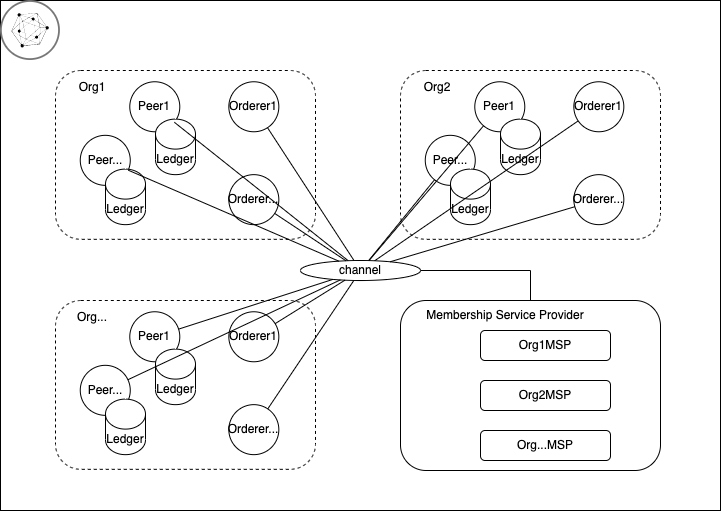
\includegraphics[width=\textwidth]{assets/pics/fabric_arch}
	\caption{Arsitektur umum aplikasi Fabric.}
	\label{fig:fabric_arch}
\end{figure}

Proses transaksi pada Hyperledger Fabric digunakan arsitektur bernama \textit{execute-order-validate}. \textit{Execute} yaitu menjalankan kemudian melakukan \textit{endorse} transaksi. Setelah \textit{endorsement policy} terpenuhi transaksi kemudian di-\textit{submit} dan diurutkan oleh \textit{ordering service} kemudian dicatat dalam \textit{block}. Setelah \textit{block} selesai dibuat kemudian \textit{block} disebarkan ke semua \textit{peer} untuk dilakukan validasi dan \textit{commit} pada \textit{ledger} masing-masing \textit{peer}.

Berbeda dengan \textit{blockchain} lain pada umumnya, pada Hyperledger Fabric seluruh kegiatan konsensus dan pembuatan \textit{block} dilakukan oleh \textit{ordering service}. Fitur modular \textit{pluggable consensus} pada Hyperledger Fabric memungkinkan untuk memilih metode konsensus yang digunakan. Sebelumnya terdapat tiga metode konsensus yang didukung oleh Hyperledger Fabric: solo untuk \textit{ordering service} dengan satu \textit{node}, kafka, dan raft. Saat ini, konsensus solo dan kafka sudah \textit{deprecated} sejak versi Fabric 2.0 dikarenakan raft lebih mendukung secara skalabilitas, dapat mencapai \textit{byzantine fault tolerance}, serta lebih transparan karena tidak perlu mengelola \textit{cluster} kafka karena hal ini menimbulkan sentralisasi pada pihak pengelola \textit{cluster} kafka. Selain itu, konsensus raft sudah tertanam dalam kode \textit{ordering service} milik Hyperledger Fabric sehingga tidak perlu melakukan konfigurasi tambahan \citep{Androulaki2018}. 

Terdapat dua cara untuk memanggil fungsi pada \textit{smart contract} yaitu memanggil metode \textbf{SubmitTransaction()} dan \textbf{EvaluateTransaction()}. \textbf{SubmitTransaction()} digunakan untuk melakukan operasi yang mengubah data dalam \textit{world state} (\textit{unsafe operation}) dan transaksi dicatat dalam blok. Sedangkan metode \textbf{EvaluateTransaction()} digunakan untuk membaca data dari \textit{world state} yang telah ter-\textit{commit} (\textit{safe operation} dan pemanggilan \textit{chaincode} hanya dilakukan secara lokal sehingga tidak melibatkan \textit{peer} lain maupun \textit{orderer} \citep{Androulaki2018}.

Sedangkan ketika metode SubmitTransaction() dipanggil, Pemanggilan fungsi dipropagasi ke semua \textit{endorsing peer} untuk dieksekusi \textit{chaincodenya} pada masing-masing \textit{endorsing peer}. Setelah mencapai kesepakatan (sesuai \textit{endorsement policy} yang ditulis dalam pengaturan \textit{channel}), transaksi dikirim ke \textit{orderer} untuk dibuatkan \textit{block}. Setelah \textit{block} dibuat \textit{block} akan dikirim ke semua \textit{peer} \citep{Androulaki2018}.

\subsection{Perbandingan \textit{Blockchain} Hyperledger Fabric dengan Ethereum}

Ethereum adalah \textit{blockchain} \textit{public permissionless} dengan pasar tertinggi selain Bitcoin \citep{Yaga2018}. Ethereum merupakan \textit{blockchain} dengan bahasa pemrograman bawaan yang \textit{turing-complete} yang memungkinkan siapapun untuk membuat aplikasi secara \textit{arbitrary} yang terdesentralisasi. Ethereum menggunakan koin \textit{cryptocurrency} bernama Ether yang digunakan sebagai biaya transaksi \citep{buterin2014next}.

Pembahasan selanjutnya adalah perbandingan antara \textit{blockchain} Hyperledger Fabric dengan Ethereum. Mohammed dkk., membuat perbandingan antara \textit{blockchain} Hyperledger Fabric dengan Ethereum \citep{Mohammed2021}. Selain perbedaan aksesibilitas (\textit{public permissionless} dengan \textit{private permissioned}), Hyperledger Fabric memiliki metode konsensus yang berbeda dengan Ethereum. Terdapat 3 metode konsensus pada Fabric yaitu solo, kafka, dan raft, yang sudah disebutkan sebelumnya. Sementara untuk Ethereum konsensus menggunakan metode Proof-of-Work. 

Perbedaan lainnya adalah tidak dibutuhkannya sebuah \textit{cryptocurrency} (namun bisa diimplementasi) pada Hyperledger Fabric dalam menggunakan \textit{smart contract}. Pada Ethereum diperlukan kegiatan \textit{mining} untuk menghidupkan jaringan, tidak halnya pada Hyperledger Fabric. Untuk pengembangan \textit{smart contract}, Hyperledger Fabric dapat diimplementasi dengan bahasa pemrograman Java, Node.js, atau Go sedangkan \textit{smart contract} Ethereum menggunakan Solidity \citep{Mohammed2021}.

Dengan terbatasnya akses untuk bergabung pada jaringan \textit{blockchain} Hyperledger Fabric serta transparansi identitas yang diberikan, Hyperledger Fabric dipilih sebagai platform \textit{blockchain} untuk mengimplementasi sistem INSW. Selain itu, dengan modularitas komponen \textit{membership service provider} anggota baru dapat dengan mudah ditambahkan ke jaringan maupun keluar dari jaringan. Ditambah lagi \textit{blockchain private} memiliki efisiensi dan kecepatan yang lebih tinggi dibandingkan \textit{blockchain} publik  \citep{Ahmad2021} dapat meningkatkan \textit{throughput} transaksi pada sistem INSW.

\section{Masalah Umum pada Aplikasi Berbasis \textit{Blockchain}}
\label{sec:masalahblockchain}

Terdapat permasalahan-permasalahan yang umum muncul pada aplikasi berbasis \textit{blockchain}. Terdapat studi \citep{Macrinici2018} yang melakukan studi pemetaan sistematis terhadap 64 publikasi ilmiah tentang aplikasi \textit{smart contract}. Metode penelitian dilakukan dengan mencari publikasi dari berbagai sumber, kemudian dilakukan penyaringan berdasarkan judul, hasil, dan kesimpulan. Dari publikasi tersebut kemudian dilakukan analisis dan klasifikasi, setelah itu pada akhirnya dilakukan pengambilan data dan pemetaan masalah.

Dalam penelitian tersebut diidentifikasi 16 masalah-masalah umum pada \textit{smart contract}. Masalah-masalah tersebut yaitu mekanisme konsensus, \textit{sacrificed performance for scalability}, \textit{unpredictable state}, \textit{generating randomness}, \textit{timestamp dependency}, \textit{lack of reimbursement}, \textit{unilateral abortion}, \textit{lack of privacy}, \textit{call to the unknown}, \textit{exception disorder}, \textit{gasless send, out of gas exception}, \textit{typecast mismatch}, \textit{re-entrancy}, pemrograman \textit{smart contract}, \textit{stack overflow}, dan \textit{cryptocurrency transfer loss}. Masalah yang paling banyak timbul adalah \textit{unpredictable State, generating randomness,} dan pemrograman \textit{smart contract}. 

Untuk masalah mekanisme konsensus dipaparkan bahwa terdapat masalah pada Proof-of-Work yang telah disebutkan pada Subsubbab \ref{subsec:consensus} yaitu konsumsi energi yang besar serta risiko sentralisasi dengan serangan 51\%. Disebutkan juga masalah pada Proof-of-Stake yaitu masalah \textit{nothing-at-stake}, penurunan keamanan, serta penghambatan penyelesaian transaksi. Meskipun risiko sentralisasi pada Proof-of-Stake lebih rendah daripada Proof-of-Work, risiko tersebut tetap ada \citep{Macrinici2018}.

Pada masalah pemrograman \textit{smart contract}, beberapa faktor keamanan perlu dipertimbangkan ketika memprogram \textit{smart contract}. Salah satunya yaitu serangan exploit Rubixi yang dapat mengancam \textit{immutability} pada sistem. Selain faktor tersebut, terdapat kesulitan dalam faktor ekonomi dalam pemrograman \textit{smart contract} yaitu biaya \textit{deploy} dan biaya transaksi untuk melakukan \textit{testing} pada \textit{smart contract} yang dibuat. Kesalahan lain terkait dengan penyimpanan yaitu pada kasus Ethereum, jika pengembang \textit{smart contract} melakukan kesalahan dan terdapat operasi \textit{write}, data tersebut akan dengan cepat terpropagasi ke ribuan \textit{node} pada jaringan.

Untuk kedua masalah mekanisme konsensus dan pemrograman \textit{smart contract} dapat diselesaikan dengan Hyperledger Fabric. Seperti yang telah disebutkan, Hyperledger Fabric menggunakan konsensus yang lebih efisien dibandingkan konsensus pada \textit{permissionless blockchain} sehingga menyelesaikan masalah konsumsi energi yang tinggi tanpa menambah risiko sentralisasi. Hal itu dikarenakan pada \textit{permissioned blockchain} masing-masing anggota berasumsi bahwa anggota lainnya dapat dipercaya dan lebih transparan. Sedangkan untuk pemrograman \textit{smart contract} pada Hyperledger Fabric tidak memerlukan biaya tambahan untuk men-\textit{deploy} aplikasi karena Hyperledger Fabric tidak mengharuskannya ada \textit{cryptocurrency} dan biaya transaksi serta dapat di-\textit{deploy} secara lokal dengan teknologi \textit{container} menggunakan Docker sehingga tidak memerlukan biaya \textit{deploy} seperti pada \textit{blockchain} publik. 

\section{Penelitian Terkait Sistem Logistik Berbasis \textit{Blockchain}}
\label{sec:penelitianlain}

Pada bagian ini, dibahas mengenai penelitian-penelitian terkait sistem logistik berbasis \textit{blockchain}. Penelitian yang pertama yaitu rancangan ulang aplikasi \textit{supply chain tracking} berbasis \textit{smart contract} dan \textit{blockchain} \citep{Chang2019}. Rancangan merupakan kombinasi sistem \textit{blockchain} dan non-\textit{blockchain} yang mengakses \textit{database} eksternal dengan perantara \textit{smart contract} yaitu \textit{query forwarder} dan \textit{query dispatcher}. Hasil penelitian mengatakan bahwa meskipun secara umum sistem \textit{database} tersentralisasi lebih efisien dalam aspek \textit{throughput} transaksi dan \textit{latency}, sistem terdesentralisasi tetap dapat mencapai efisiensi yang \textit{practically acceptable}. Konfigurasi-konfigurasi \textit{blockchain} lain seperti platform \textit{blockchain}, protokol konsensus, komputasi dan penyimpanan data \textit{on-chain/off-chain}, ukuran \textit{block}, dan derajat sentralisasi dapat dilakukan eksplorasi lebih lanjut dalam upaya meningkatkan efisiensi.

Penelitian selanjutnya adalah rancangan sistem \textit{port supply chain} berbasis \textit{blockchain} Fabric bernama Fabric-PSChain \citep{Gao2022}. Terdapat enam \textit{user role} pada aplikasi ini yaitu \textit{consignor}, \textit{forwarder}, \textit{shipping company}, \textit{port}, \textit{consingee}, dan \textit{regulator}. Sistem menerapkan \textit{Role-Based Access Control Policy} (RBACP) agar \textit{user} terotentikasi sehingga informasi-informasi yang diterima \textit{user} sesuai berdasarkan \textit{role user} tersebut. Konsensus \textit{node} mencegah pengunggahan informasi palsu dengan cara setengah atau lebih \textit{node} harus memvalidasi suatu informasi, jika tidak maka informasi tersebut tidak akan ditulis ke dalam \textit{ledger} sehingga hal ini mencegah perusahaan mengubah data sembarangan dan meningkatkan reliabilitas transaksi. Sistem penyimpanan yang terdistribusi juga melindungi dari perusakan data tanpa wewenang dan meningkatkan integritas data.


Penelitian lainnya adalah penelitian mengenai aplikasi dan arsitektur \textit{blockchain} untuk operasi dan manajemen logistik pelabuhan \citep{Ahmad2021}. Penelitian ini mengajukan dan membandingkan arsitektur sistem operasi pelabuhan menggunakan Hyperledger Fabric dengan Hyperledger Besu. Kedua platform \textit{blockchain} tersebut dapat menjaga kerahasiaan data dengan komunikasi secara privat. Fitur privasi dari arsitektur yang diajukan dapat mengatasi masalah ketika para \textit{stakeholder} tidak sepenuhnya mempercayai satu sama lain. Dikatakan juga bahwa proses transaksi dengan Hyperledger Fabric dan Hyperledger Besu lebih cepat diselesaikan dibandingkan dengan platform \textit{blockchain} publik.
